\chapter{Results}
The first result is of course a working CAK subroutine and FLD module in \texttt{MPI-AMRVAC}. This is something that didn't exist before and it will open the way toward simulations of new physical regimes where radiation plays a role in the dynamics of the system. In addition to   designing, writing and benchmarking the software, there are also a few first scientific results. These will be described in this chapter.

\section{CAK-Theory}
\subsection{Massive Star Stellar Wind}
The CAK momentum equation for a point like star, so when disregarding the finite disk correction factor, has an analytic solution. This solution will be derived below, based on \citep{Owocki2003}, for comparison with the numerical models. Afterwards, the corrections for finite disks will be mentioned. Begin by writing down the steady state momentum equation in 1D spherical coordinates, disregarding the pressure term. The pressure gradient will be orders of magnitude smaller than the gravitational and radiative accelerations due to the low density environment. 
\begin{align}
\nabla_r \left(v_r \rho v_r \right) = \rho g_{CAK} + \rho g_{e} - \rho g_{grav}
\end{align}
Using the steady state continuity equation and the electron scattering Eddington factor $\Gamma_e$ this can be written as:
\begin{align}
v \frac{d v}{d r} = g_{CAK} + (\Gamma_e-1) \frac{G M_*}{r^2} \label{eq: CAK_mom}
\end{align}
Lets introduce two new variables: $x = 1- \frac{R_*}{r}$ is a dimensionless inverse radius coordinate, and $w = \frac{v^2}{v_{esc}^2}$ is the kinetic energy as ratio of the kinetic energy at effective escape velocity. The effective escape velocity is similar to the general expression for escape velocity, but corrected for electron scattering force: $v_{esc} = \sqrt{(1- \Gamma_e) \frac{2 G M_* }{R_*}}$. Using the notation $w' = \frac{dw}{dx} = \frac{dw}{dr}\frac{dr}{dx}$ and $v' = \frac{dv}{dx} = \frac{dv}{dr} \frac{dr}{dx}$, equation \eqref{eq: CAK_mom} can be written as:
\begin{align}
w' &= C w'^\alpha - 1 \label{eq: CAK_w}
\end{align}

Where, if we define the constant mass loss rate $\dot{M} = 4\pi r^2 \rho(r) v(r) = c^{ste}$, C is given by:
\begin{align}
C = \frac{1}{1-\alpha} \left(\frac{\bar{Q}\Gamma_e}{1-\Gamma_e} \right)^{1-\alpha} \left(\frac{L_*}{\dot{M}c^2}\right)^\alpha \label{eq: CAK_Cste}
\end{align}
$C$ Depends inversely on the mass loss rate $\dot{M}$, depending on the value of $C$, equation \ref{eq: CAK_w} has either zero ($C < C_{crit}$), one ($C = C_{crit}$) or two ($C = C_{crit}$) solutions. A low value for $C$ leads to a high $\dot{M}$, so the solution with the maximal mass loss rate is the single solution at $C = C_{crit}$ The critical value for $C$ occurs when the function $C w'^\alpha$ intersects function $1 + w'$ in a tangent point. This occurs at critical argument $w'_{crit} = \frac{\alpha}{1-\alpha}$ for critical $C$-value $C = \frac{\alpha^{-\alpha}}{(1-\alpha)^{1-\alpha}}$. One can now integrate over $w'_{crit}$ to obtain a velocity profile.
\begin{align}
w'_{crit} &= \frac{\alpha}{1-\alpha} \\
v(r) &= v_{esc} \sqrt{\frac{\alpha}{1-\alpha}} \left(1 - \frac{R_*}{r} \right)^\frac{1}{2}
\end{align}
Where, when $r\rightarrow\infty$, $v(\infty) \rightarrow v_{esc} \sqrt{\frac{\alpha}{1-\alpha}} = v_\infty$. This type of velocity field follows a beta velocity law ($v = v_\infty (1-R/r)^\beta$), where in this case $\beta = 0.5$. The maximal CAK mass loss rate connected to the critical value $C_{crit}$ can also be analytically determined by solving equation \ref{eq: CAK_Cste} for $\dot{M}$:
\begin{align}
\dot{M}_{CAK} = \frac{L_*}{c^2} \frac{\alpha}{1-\alpha}\left(\frac{\bar{Q}\Gamma_e}{1-\Gamma_e}\right)^{\frac{1-\alpha}{\alpha}}
\end{align}

Let's now have a look at some corrections that can be made when considering a finite disk instead of a point source. Define the rescaled correction factor as $f_* = \frac{f_{fd}}{f}$ and the rescaled constant $C_* = C f$, where $f$ is the finite disk correction factor at the stellar surface. At the stellar surface, $r \rightarrow R_*$, $v \rightarrow 0$ and $dv/dr \sim v/r$, plug this in in equation \ref{eq: fin_disk_corr} gives $f_{fd}(R_*) = f \sim \frac{1}{1+\alpha}$. Equation \ref{eq: CAK_w} now rescales to:
\begin{align}
w' = f_* C_* (w')^\alpha - 1 \label{eq: w_fd}
\end{align}
Analogous reasoning as before leads to an adjusted CAK mass loss rate $\dot{M}_{fd}$. This mass loss rate will be lower than the point source mass loss rate, because $f \sim \frac{1}{1+\alpha}  < 1$.
\begin{align}
\dot{M}_{fd} = \frac{\dot{M}_{CAK}}{(1+\alpha)^\frac{1}{\alpha}}
\end{align} 


Now that we have testable observables (the steady state CAK mass loss rate $\dot{M}_{CAK}$ and the steady state velocity and density profiles $v(r), \rho(r)$), it is time time to run some simulations and compare the outcomes to the analytical solutions.\\

The CAK source term is used to model the wind of a massive O-type star. A star of luminosity $L = 8\cdot 10^5 L_\odot$ and mass $M = 50 M_\odot$ is taken at as the mass driver (see table \ref{tab: CAK_res}). \\

\begin{table}[]
\centering
\caption{Top part: Parameters used in setting the initial conditions of the wind based on \citep{Sundqvist2013}. Bottom part: Fitted parameters.}
\label{tab: CAK_res}
\begin{tabular}{llll}
\hline
\hline
\multicolumn{4}{l}{Stellar wind parameters}                                           \\
\hline
$R/R_\odot$              &             & $20$ &\\
$L/L_\odot$              &             &  $8\cdot10^{5}$  &\\
$M/M_\odot$              &             & $50$ &\\
$T[K]$                   &             & $4\cdot10^{4}$ &\\
$c_{adiab}[\frac{m}{s}]$ &             & $2.3\cdot 10^{6}$ &\\
$\bar{Q}$ 				 &             & $2000$ &\\
$\alpha$                 &             & $0.67$ &\\
$\rho_0[\frac{g}{cm^3}]$ &             & $2.2\cdot 10^{-12}$ &\\
\hline
\hline
\multicolumn{4}{l}{Fitting parameters}                                                \\
                         & theoretical & best fit point source & best fit finite disk \\
\hline
$\beta$                  & $0.5$       & $0.543\pm 0.001$      &  $0.761 \pm 0.001$   \\
$v_{\infty}/c_{adiab}$   & $45.69$     & $33.14\pm 0.04$       &  $149.4 \pm 0.1$     \\
$\dot{M}_{CAK}[\frac{M_\odot}{yr}]$ & $4.1 \cdot 10^{-6}$  & $(3.4 \pm 0.4)10^{-7}$&  $(1.8\pm0.2)10^{-7}$ \\           
\end{tabular}
\end{table}


The tricky bit in the setup of this simulation is choosing correct lower boundary conditions. The stellar wind is launched from the stellar surface and begins with a subsonic velocity. Computationally this is controlled by setting the lower boundary density $\rho_0$. If the density on the lower bound is too high, the simulation domain begins "too deep" in the stellar atmosphere, the equations become too stiff \citep{Sundqvist2013}. If $\rho_0$ is too low, the simulation domain begins in the supersonic region.\\

As initial condition, the velocity field is taken as a beta velocity law with $\beta > 0.5$, this leads to higher velocity and thus a supercritical solution. The initial density can be derived from the mass los rate: $\rho = \frac{\dot{M}_{CAK}}{4\pi r^2 v}$. The velocity profile should relax towards the critical solution where $\beta = 0.5$ for the point source driven wind. For a point source, equation \eqref{eq: CAK_w} is spatialy independent, so a simple analytic integration led us to this simple velocity law. In equation \eqref{eq: w_fd} on the other hand, $f_*$ depends on $r$. Integration isn't simple, but after a few assumptions one can find $\beta = 0.8-1$ and $v_{\infty} \sim v_{esc} C_c f_*^{\frac{1}{2(1-\alpha)}} $ \citep{Owocki2003} for the finite disk driven wind. \\

The lower boundary for the radial velocity is set according to the continuity equation $\nabla (\rho v) = 0$, meaning $v_0 = \frac{\rho_1 v_1}{\rho_0}$. Initial conditions are evolved towards an almost stable, nearly steady state, results of the simulations and their analytical counterparts are plotted in figures \ref{fig: CAK_PS_v} and \ref{fig: CAK_PS_rho}.\\

A beta-velocity law is fitted trough the numerical velocity profile to get the wind characteristics. The actual mass loss rate can be calculated by fitting $\rho_{fit} = \frac{\dot{M}}{4\pi r^2 v_{fit}}$ to the density profile with $\dot{M}$ as a free parameter. Results are tabulated in table \ref{tab: CAK_res}

\begin{figure}
\centering
\begin{subfigure}{.8\textwidth}
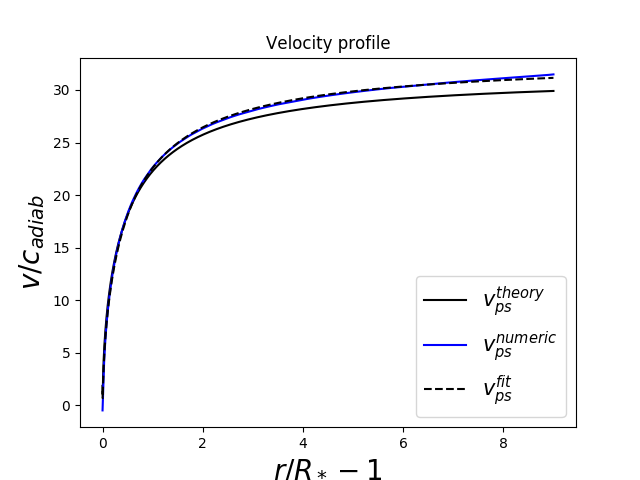
\includegraphics[width = \textwidth]{CAK_velocity_profile.png}
\caption{Velocity profile}
\label{fig: CAK_v}
\end{subfigure}
\begin{subfigure}{.8\textwidth}
\centering
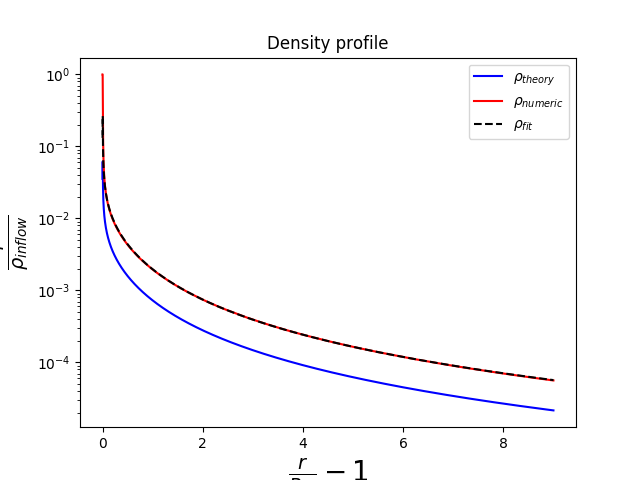
\includegraphics[width = \textwidth]{CAK_density_profile.png}
\caption{Density profile}
\label{fig: CAK_rho}
\end{subfigure}
\caption{The velocity and density profiles for the point source CAK wind. In a black solid lines the analytical solution with $\beta = 0.5$, in a blue solid line the numerical steady state solution and black in dashed lines the fitted curve trought the numerical solution.}
\label{•}
\end{figure}

When accounting for the finite disk correction, the steady state velocity profile doesn't follow a $\beta = 0.5$ velocity law, results are shown in figures \ref{fig: CAK_PS_v} and \ref{fig: CAK_PS_rho}, the correction factor is plotted in figure \ref{fig: fd_factor}. 

\begin{figure}
\centering
\begin{subfigure}{.8\textwidth}
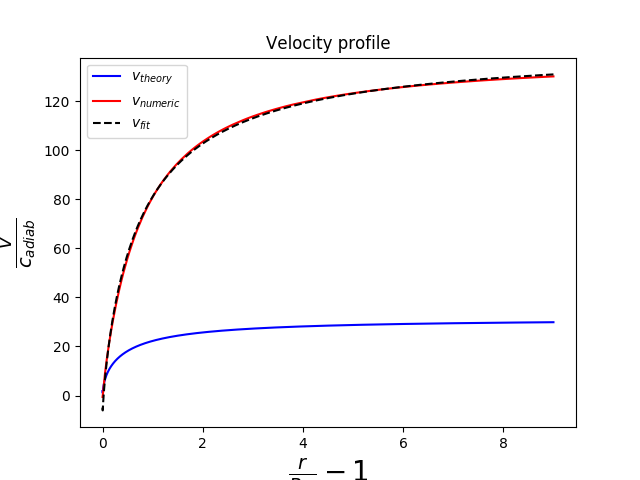
\includegraphics[width = \textwidth]{CAK_fd_velocity_profile.png}
\caption{Velocity profile}
\label{fig: CAK_fd_v}
\end{subfigure}
\begin{subfigure}{.8\textwidth}
\centering
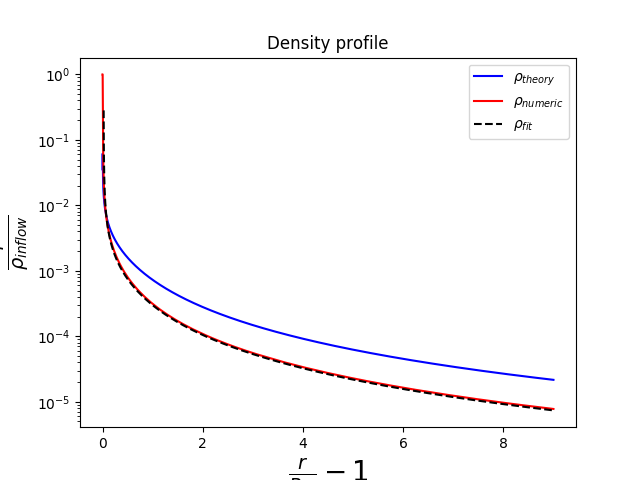
\includegraphics[width = \textwidth]{CAK_fd_density_profile.png}
\caption{Density profile}
\label{fig: CAK_fd_rho}
\end{subfigure}
\caption{The velocity and density profiles for the finite disk corrected overlayed on those for the point source CAK wind.  In a black solid lines the analytical solution with $\beta = 0.5$, in a blue solid line the numerical steady state solution and black in dashed lines the fitted curve trought the numerical solution. The red solid line is the numerical steady state with finite disk and fitted trough this is the green dashed line.}
\label{•}
\end{figure}
%
%
%\begin{figure}
%\centering
%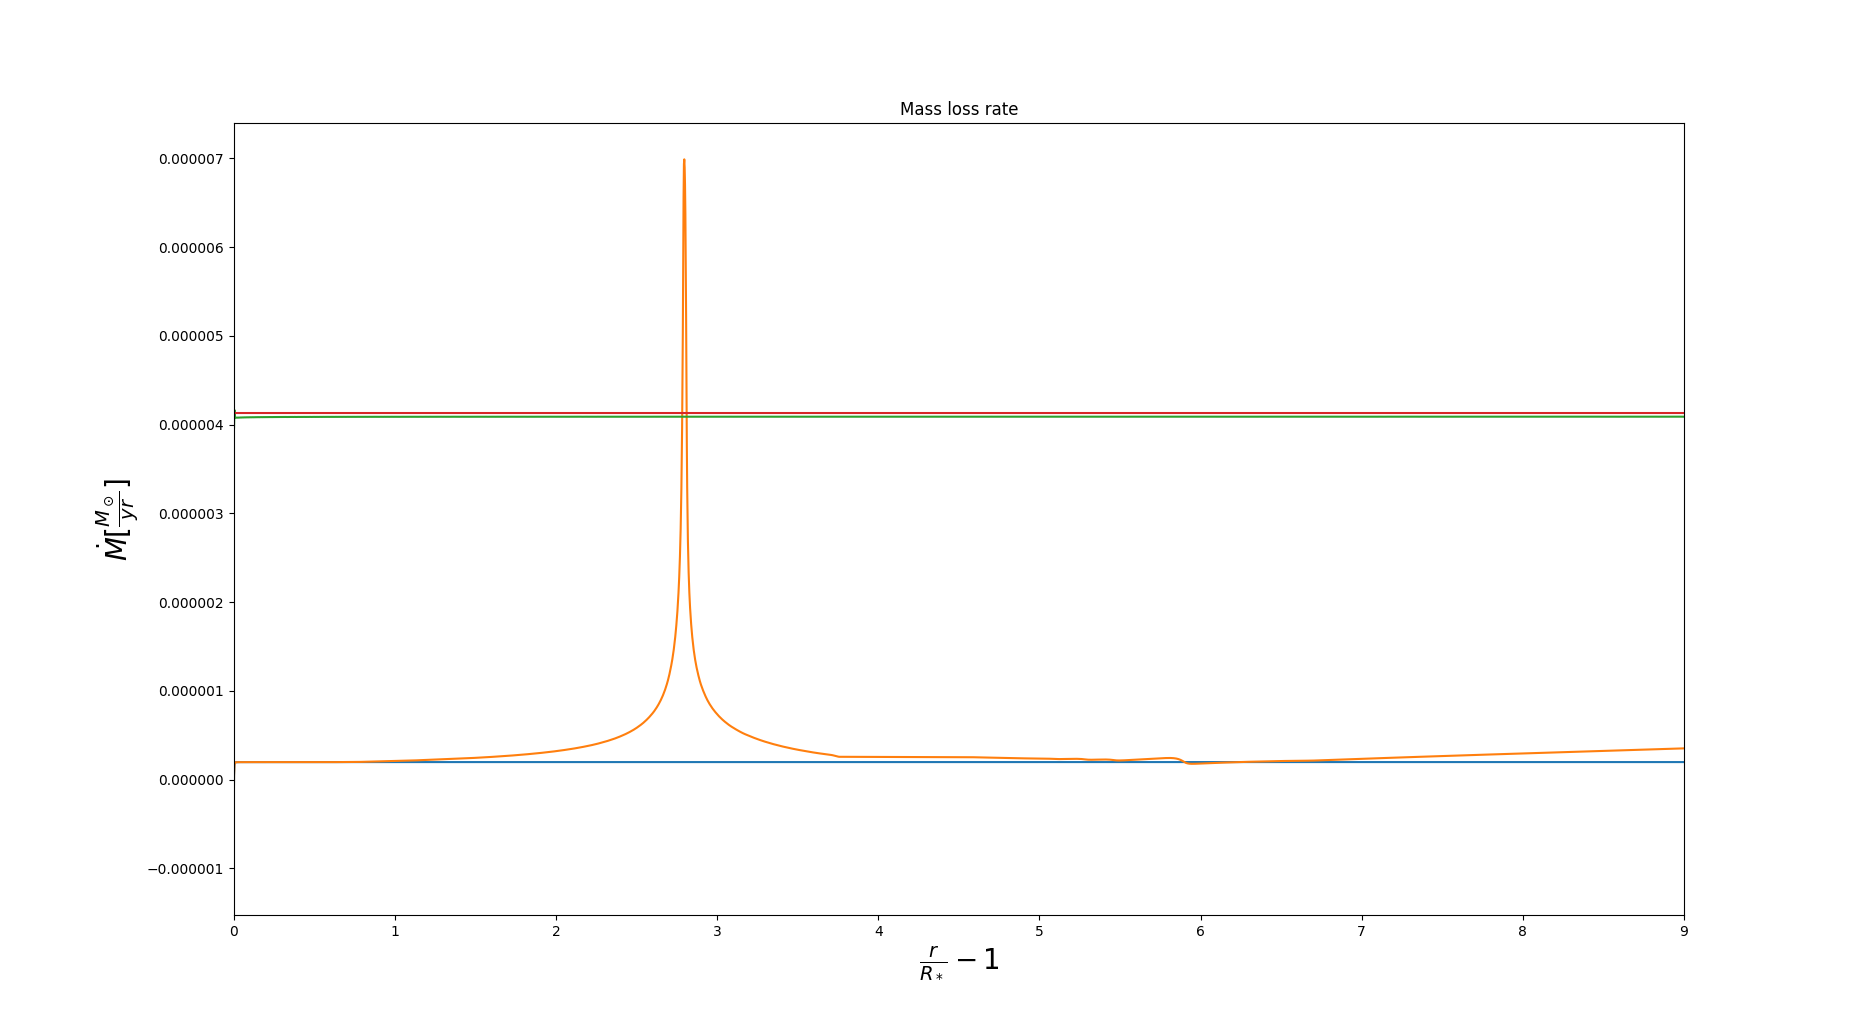
\includegraphics[width = \textwidth]{CAK_fd_mass_loss.png}
%\caption{The mass loss rate profile for the finite disk corrected CAK wind. In dashed lines the initial conditions, in green the analytical steady state solution and in blue and red the solutions after 0.5 and 50 times $t = R_*/c_{adiab}$.}
%\label{fig: CAK_fd_M_dot}
%\end{figure}

\begin{figure}
\centering
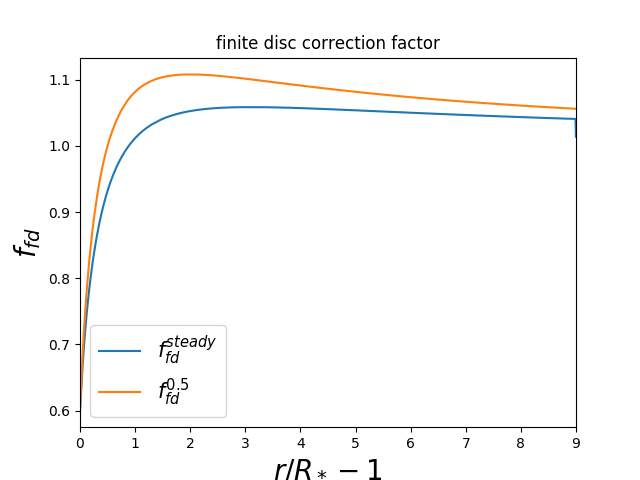
\includegraphics[width = 0.8\textwidth]{CAK_fd_factor.png}
\caption{The finite disc correction factor for the steady state solution and for a $\beta = 0.5$ velocity law.}
\label{fig: fd_factor}
\end{figure}

%Closing
Having now succesfully implemented and benchmarked a radiative line driving module into \texttt{MPI-AMRVAC}, future work will be done in for exemple extension toward 2D and 3D simulations,  interaction of stellar winds with orbiting compact objects such as BH's, NS's or WD's (X-ray binaries) \citep{Mellah2017}.


\section{Flux Limited Diffusion}
The diffusion model is first tested against some analytical results, these tests will give us knowledge on how accurately we can interpret the simulations of physical phenomena. The diffusion term and advection term are both tested separately by comparison to an exact solution and the photon tiring, radiative cooling and radiative heating source terms are tested together versus a Runge-Kutta solver of a simplified problem.

\subsection{Testcase 1: Advection and Diffusion}\label{section: res: diff_test}
The advection problem and the diffusion problem, solved by the already existing Riemann solver and the new ADI solver respectively can be tested by comparing them to simplified situation where an exact analytical solution can be found. The Riemann solver is nothing new, it's just a matter of checking the correct implementation in \texttt{MPI-AMRVAC}. The problem is tested on a numerical domain with constant density, a constant velocity, a constant gas energy density and an initial radiation energy density $E_0(x,y,t)$ given by:
\begin{align}
E_0(x,y,t) = 2 + \sin(2 \pi x) \sin(2 \pi y)
\end{align}
If diffusion and other source terms are ignored, the radiation field will evolve as
\begin{align}
E^{adv}(x,y,t) = 2 + \sin(2 \pi (x-v_x t)) \sin(2 \pi (y-v_y t))
\end{align}
If diffusion is switched on but the advection is ignored by fixing the velocity field to $\vec{0}$ every iteration, and the diffusion coefficient is chosen constant at $D = 1$, the field evolves as
\begin{align}
E^{diff}(x,y,t) = 2 + \exp(-8 \pi^2 t) \sin(2 \pi x) \sin(2 \pi y)
\end{align}

Function $E_0(x,y,t)$ describes a series of dots of more and less radiative energy, see figure \ref{fig: InitCond_test}. The numerical domain is chosen in such a way that there is one region of lower and one region of higher energy in each direction, $-0.5 \leq x \leq 0.5$, $0 \leq y \leq 1$. In time, the diffusion test runs until the amplitude of the dots diminish by two orders of magnitude $\exp(-8 \pi^2 t)  = 10^{-1}$ and the advection test tuns until a point has passed the computational domain twice $ \min(v_x, v_y) t = 2 $. Boundary conditions are set periodical. Computational result $\tilde{E}$ can be compared with the analytical results to define the residuals:
\begin{align}
RES^{adv} &= \left|\frac{\tilde{E}^{adv} - E^{adv}}{E^{adv}}\right| \\
RES^{diff} &= \left|\frac{\tilde{E}^{diff} - E^{diff}}{E^{diff}}\right| 
\end{align}

\begin{figure}
\centering
\includegraphics[width = 0.6\textwidth]{InitCond_test.png}
\caption{The initial conditions radiation energy density for the advection and diffusion test cases.}
\label{fig: InitCond_test}
\end{figure}

Which are plotted for different timesteps in figure \ref{fig: test_advection} and \ref{fig: test_diffusion} together with the numerical solutions $\tilde{E}^{adv}$ and $\tilde{E}^{diff}$


\begin{figure}
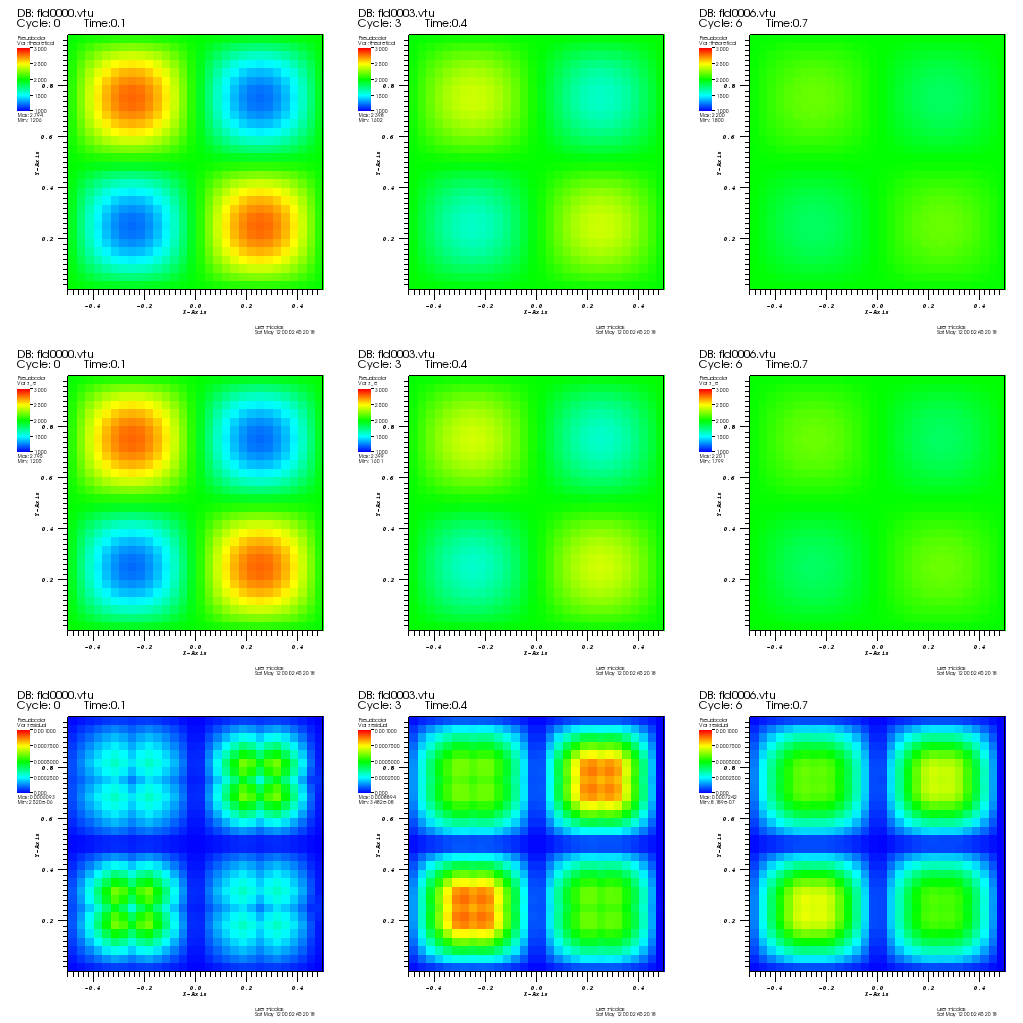
\includegraphics[width = \textwidth]{visit0001.png}
\caption{top: theoretical solution $E^{diff}$, middle: computed result $\tilde{E}^{diff}$ and bottom: residual $RES^{diff}$. Left: $0.1 t_0$, middle $0.4 t_0$ and right $0.7 t_0$. The color scale goes from $1$ (blue) to $3$ (red) for the upper two rows and form $0$ (blue) to $0.01$ (red) for the bottom row.}
\label{fig: test_diffusion}
\end{figure}

\begin{figure}
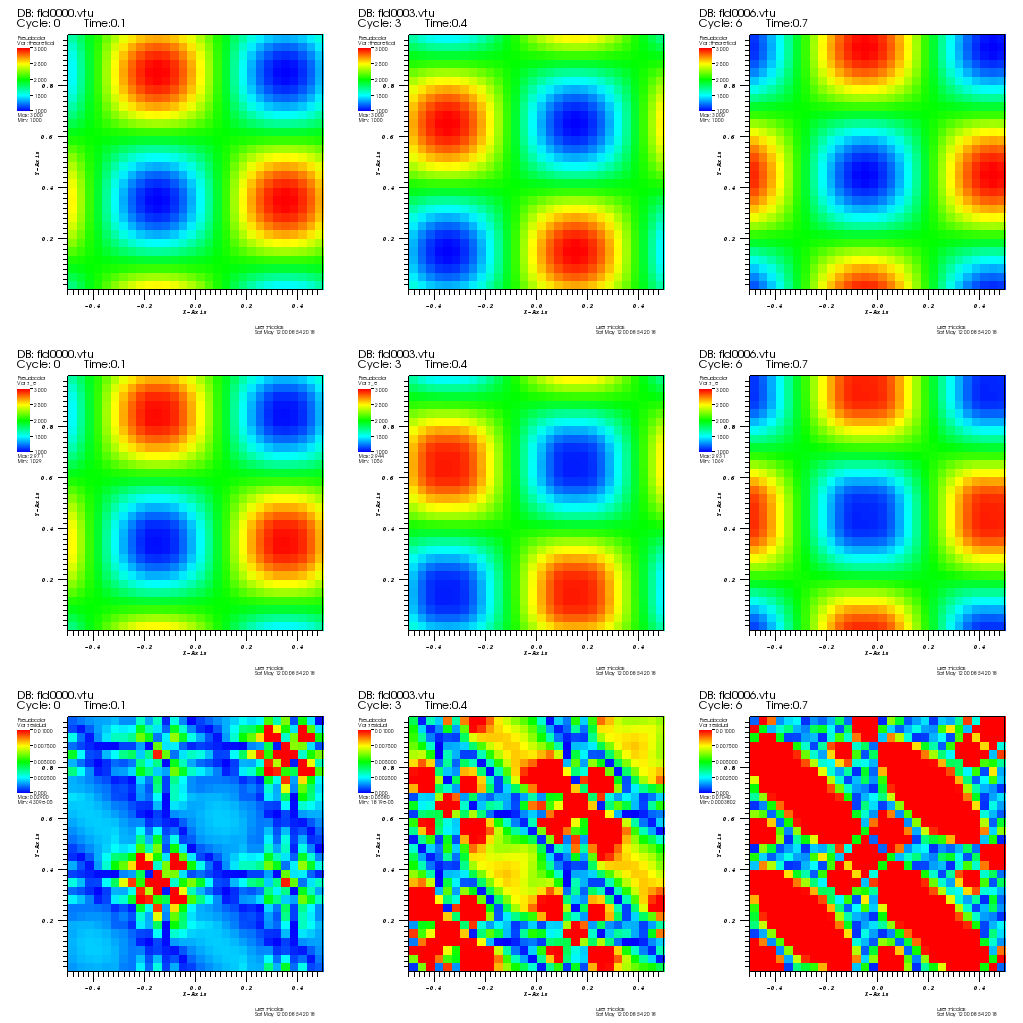
\includegraphics[width = \textwidth]{visit0002.png}
\caption{top: theoretical solution $E^{adv}$, middle: computed result $\tilde{E}^{adv}$ and bottom: residual $RES^{adv}$. Left: $0.1 t_0$, middle $0.4 t_0$ and right $0.7 t_0$. The scale goes from $1$ to $2$ for the upper two rows and form 0 to 0.001 for the bottom row.The color scale goes from $1$ (blue) to $3$ (red) for the upper two rows and form $0$ (blue) to $0.001$ (red) for the bottom row.}
\label{fig: test_advection}
\end{figure}



\subsection{Testcase 2: Photon Tiring, Heating and Cooling}
To test the implicit bisection scheme used for adding the photon tiring, radiative heating and radiative cooling source terms, we make comparisons with an explicit Runge-Kutta solver. Of course this Runge-Kutta solver is not to be used in the actual code, because the time step chosen in the Runge-Kutta solver will be orders of magnitude smaller. The equation at hand is:
\begin{align}
\frac{d e}{dt} = c \rho \kappa E - 4 \rho \kappa \sigma T^4
\end{align}
Equivalently the test can be ran on the source terms for the radiative energy equation $\frac{dE}{dt} = - \vec{\nabla} \cdot \vec{v} P + 4\pi \kappa\rho B - c \kappa \rho E$ , where the photon tiring term would drop out due to the velocity field being zero.
Except for the gas energy density, all primitive variables ($\rho = \rho_0$, $\vec{v} = 0$ and $E = E_0$) are kept constant. The computational domain is taken as small as possible and radiative diffusion is switched off. \\

The system would be in radiative equilibrium when $c \rho \kappa E = 4 \rho \kappa \sigma T^4$. Using $T =  \frac{p}{\rho} \frac{m_p \mu}{k_b}= \frac{(\gamma - 1)e}{\rho} \frac{m_p \mu}{k_b}$, on can compute the equilibrium gas energy.
\begin{align}
e_{eq.} = \frac{\rho}{\gamma - 1} \frac{k_b}{m_p \mu}\left( \frac{c E}{4 \sigma} \right)^\frac{1}{4}
\end{align}
Different initial conditions are chosen for $e_0$ ranging from $10^2 e_{eq.}$ to $10^{-10} e_{eq.}$. Comparisons between the bisection method and a simple fourth order Runge-Kutta solver are plotted in figure \ref{fig: test_sourceterms} for different initial energy conditions, and in figure \ref{fig: test_sourceterms_dt} for different time steps. Remember that the implicit bisection method uses a time step which is several orders of magnitude larger than the explicit Runge-Kutta method.

\begin{figure}
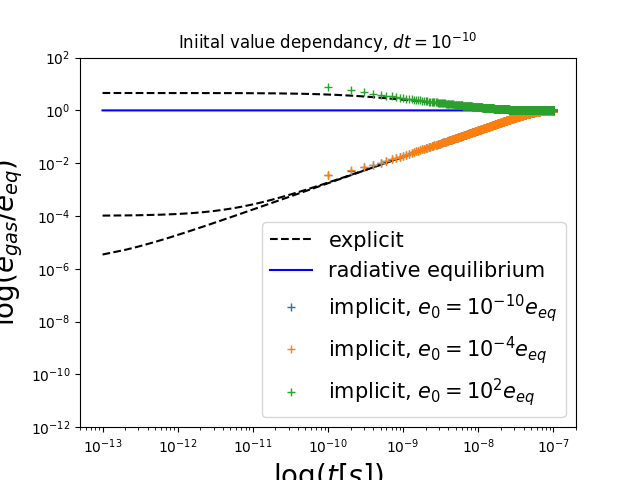
\includegraphics[width = \textwidth]{test_sourceterms.png}
\caption{Comparison between the implicit method in red crosses and explicit method in a black dashed line for computing the radiation heating and cooling sourceterms. The gas energy evolves toward radiative equilibrium (blue) from different initial values. The time step for the implicit method is 3 orders of magnitude larger than the time step for the explicit method.}
\label{fig: test_sourceterms}
\end{figure}

\begin{figure}
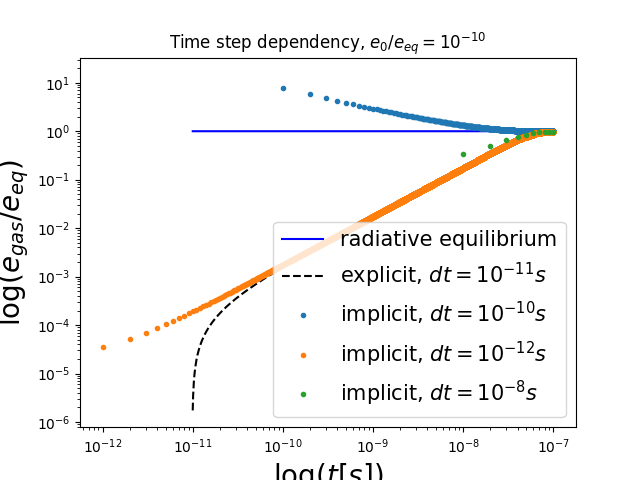
\includegraphics[width = \textwidth]{test_sourceterms_dt.png}
\caption{Comparison between the implicit method in orange, blue and green dotted lines and explicit method in black dashed lines for computing the radiation heating and cooling sourceterms. The gas energy evolves toward radiative equilibrium (blue) with different time steps for the implicit method.}
\label{fig: test_sourceterms_dt}
\end{figure}

\subsection{Isothermal Thomson Atmosphere} \label{section: IsoAtm}
A first practical use for the FLD module is modelling a stellar atmosphere surrounding a massive star. For convenience, the atmosphere will be considered isothermal and plane parallel, so the flux in the initial condition and the gravitational acceleration are constant. Let's also assume the only absorption an emission is done by means of electron scattering (Thomson atmosphere), with a constant opacity $\kappa$. The model is done in 2D. To find suitable initial conditions, which are crucial in stabilizing simulations, lets begin by writing down the hydrostatic equation \eqref{eq: hydrostatic}. In a steady state, when the velocity field is constant, the momentum equations turns to:\\
\begin{align}
\frac{dp}{dy} = -g_{eff} \rho \label{eq: hydrostatic}
\end{align}
This equation describes a regime where the effective gravitational acceleration ($g_{eff} = g_{grav} - g_{rad} = g_{grav}(1 - \Gamma)$) is countered by the pressure gradient, the velocity field is $\vec{0}$ everywhere. In an isothermal atmosphere, the density and gas pressure decay exponentially on the length of a pressure scale height $H_{eff} = \frac{c_{sound}^2}{g_{eff}}$. 
\begin{align}
\rho(y) &= \rho_0 \exp \left( -\frac{y}{H_{eff}} \right) \\
 p(y)   &= p_0    \exp \left( -\frac{y}{H_{eff}} \right)
\end{align}

Now, the boundary conditions $\rho_0$ and $p_0$ have to be computed. Consider the integrated density from a  spatial coordinate $y'$ until $\infty$ to be the column mass at $y'$: $m_{col}(y') = \int^\infty_{y'} \rho(y) dy$. Filling this in the hydrostatic equation gives an expression for the pressure $p(y')$ at point $y'$.
\begin{align}
p(y') = -g_{eff} m_{coll}(y')
\end{align}
An important quantity in the study of stellar atmospheres is the optical depth $\tau$, which can be defined as the length integral over the absorption coefficient $\tau(y') = \int_\infty^{y'} \kappa \rho(y) dy$. Or, making use of the column mass and a constant opacity:
\begin{align}
\tau(y') = -\kappa m_{col}(y') \label{eq: opt_depth}
\end{align}
At any optical depth, the pressure can be written as: 
\begin{align}
p = g_{eff}\frac{\tau}{\kappa}
\end{align}
So instead of selecting a boundary condition in coordinate-space, a boundary condition is selected by choosing a value $\tau_0$ in optical depth-space. The boundary condition for the gas pressure is set by $p_0 = g_{eff}\frac{\tau_0}{\kappa}$, and using the isothermal speed of sound, the boundary condition for mass density is $\rho_0 = 0/c_{sound}^2$. In a static medium, the gravitational and radiative acceleration of the gas is countered by the gas pressure gradient. Concerning the radiation field, one can make a similar statement. The radiative acceleration is countered by the radiation pressure gradient:
\begin{align}
\frac{dp}{dy} \frac{1}{\rho} &= \frac{dp}{dm} = -g_{grav}(1 - \Gamma) \label{eq: p_cond} \\
\frac{dP}{dy} \frac{1}{\rho} &= \frac{dP}{dm} = -g_{grav} \Gamma \label{eq: P_cond}
\end{align}
\eqref{eq: P_cond} And \eqref{eq: p_cond} can by divided by one another to get a relation between $dp$ and $dP$. Integrate to find a lower value for the radiation pressure.
\begin{align}
dP = \frac{\Gamma}{\Gamma-1} dp \\
P_0 = \frac{\Gamma}{\Gamma-1} p_0
\end{align}
The gas energy density can be set from the gas pressure profile. Because of a constant initial flux (the plane parallel approximation) and a constant opacity, $\Gamma$ is constant as well and in the Eddington limit, $E=3P$. Now we have a boundary condition for the radiation energy field as well. The initial conditions are given by:
\begin{align}
\rho(y) &= g_{eff} \frac{\tau_0}{\kappa c_{sound}^2} \exp \left( -\frac{y}{H_{eff}} \right) \\
\rho \vec{v} &= \vec{0} \\
e &= \frac{\tau_0}{\kappa (\gamma - 1)} \exp \left( -\frac{y}{H_{eff}} \right) \\
E &= \frac{3 \Gamma}{1-\Gamma} \frac{\tau_0}{\kappa} \exp \left( -\frac{y}{H_{eff}} \right) \\
\end{align}

$\rho_0$ And $p_0$ are also used as lower boundary conditions for density and gas energy during the simulations. The  boundary condition for the $x$-component of the velocity is $0$ and the one for the $y$-component is set with the help of the steady state continuity equation $\partial_y(v_y \rho) = 0$. In a discrete form this can be written as:
\begin{align}
v_{y,0} = \frac{v_{y,1} \rho_1}{\rho_0}
\end{align}
Where the value in the first ghostcell is indicated with index $_0$.\\
For the radiation energy it is not only important that $E$ has the correct value, even more important is the value for $F_y$. Lets begin by writing down a discrete form of the initial conditions:
\begin{align}
E_{i+1} &= \frac{3 \Gamma_{i+1}}{1-\Gamma_{i+1}}_{i+1} \\
\Gamma_{i+1} &= \frac{1}{1 + \frac{3 p_{i+1}}{i+1}} \label{eq: Gamma1}
\end{align}
Using the defenition of the Eddington parameter $\Gamma_{i+1} = \frac{\kappa F_{y,i+1}}{c g_{grav}}$ and a discrete form of the fld closure relation equation \eqref{eq: fld_closing} $F_{i+1} = -\frac{c \lambda_{i+1}}{\kappa \rho_{i+1}} \frac{E_{i+2} + E_{i}}{2 \Delta y}$ one can write down another expression for $\Gamma$:
\begin{align}
\Gamma_{i+1} = \frac{\lambda_{i+1}}{g_{grav}\rho_{i+1}}\frac{E_i + E_{i+2}}{2 \Delta y} \label{eq: Gamma2}
\end{align}

Eliminating the Eddinton parameter in equations \ref{eq: Gamma1} and \eqref{eq: Gamma2} makes it possible to give an elegant expression for $E_i$:
\begin{align}
E_i = E_{i+2} + \frac{2 \Delta x}{1 + \frac{3 p_{i+1}}{i+1}}  \frac{g_{grav} \rho_{i+1}}{\lambda_{i+1}}  
\end{align}
This expression gives a radiation energy field which leads to a physical flux when calculating it from the closure relation. On the lower boundary, a "no inflow" condition is used. This means that the gradient of the densities is preserved as long as it is smaller than $0$. Periodic boundary conditions are used on the sides. \\ 

After every time step, the gas energy density is set as function of the gas density and momentum to match the constant temperature structure to keep the atmosphere isothermal. This is done using the inner boundary condition module in \texttt{MPI-AMRVAC}.\\

The parameters defining the physics of the system are the Eddington parameter $\Gamma$, the optical depth at the lower boundary $\tau_0$ and the sound speed $c_{sound}$. The Eddington parameter contains information about the mass, luminosity and radius of the star, it determines whether the atmosphere will be blown away, collapsing in on itself or relax in a steady state. $\tau_0$ Sets the physical lower boundary of the numerical domain. A high value means the model starts at in a high density environment near the core, a low value means the model simulates the outermost boundaries of the star. The sound speed determines the temperature of the atmosphere and the velocity at which waves can travel. Together with the Mass which sets the gravitational field, the sound speed also determines the scale height of the gas. \\

Calculations are done on a Cartesian grid, with the y-direction parallel to the radius of the star. The mass of the star is chosen at $M_* = 150 M_\odot$. Using Leavit's law, we get a luminosity for a typical $50M_\odot$ star of $L_* = 3.375 \cdot 10^{6} L_\odot$ and an Eddington parameter $\Gamma = 0.58$. The calculation domain begins at $\tau_0 = 100$ and the grid resolves about $4$ scale heights in the y-direction and $2$ in the x-direction. The resolution of the grid is chosen such that there are $10$ cells per scale height. The simulation stops after $5$ times the hydrodynamical timescale, this is the time needed for a sound wave to travel across the pressure scale height. This is more than enough time for waves to cross the entire numerical domain. In the initial conditions, a random perturbation is applied to the density of about $5 \%$.\\  

\subsection{Kramers' opacity and opacity bump}
As a first approximation, the mean opacity was assumed to be constant as function of temperature and density. In reality however, this is not the case. Numerous research groups have invested time in calculating mean opacities in different regimes, the OPAL project \citep{Iglesias1996} being one of them. In future work, one could implement a subroutine that calls value form the OPAL opacity tables. For now, two simplified cases are implemented and their effect tested on the evolution of the atmosphere: Kramers' opacity law and an opacity bump.

\begin{itemize}
\item \textbf{Kramers' opacity law:} Already in 1923, Dutch physicist Hendrik Kramers derived a parametrised expression for free-free or bound-free dominated regimes \citep{Carroll1996}:
\begin{align}
\kappa(\rho,T) = \kappa_0 \frac{\rho}{\rho_0} \left(\frac{T}{T_0}\right)^{-\frac{7}{2}}
\end{align}
A similar opacity law is implemented, where $\kappa$ and $\rho_0$ are chosen in such a way that the entire simulation domain starts of sub-Eddington ($\Gamma < 1$). For the isothermal wind, $T = constant$, and is thus not relevant for the calculations. $T_0$ is set to the atmospheric temperature. \\


\item \textbf{Opacity bump:} When considering OPAL opacities at massive star stellar atmosphere conditions, a prominent feature is the \emph{Iron opacity bump} \citep{Owocki2014} (fig: \ref{fig: opacity_bump}). The opacity increases and decreases  as a function of temperature, especially for at high densities. This is due to the number of absorption lines in iron after being ionised at about $2 \cdot 10^5 K$. In the atmospheres of massive, near Eddington limit stars, this opacity bump results in a local rise of opacity and thus a local super Eddington region. This in turn can lead to a density inversion and possibly the inflation of stellar atmospheres and the driving of stellar winds \citep{Petrovic2006}.\\

A similar feature is imitated in the code by adding a Gaussian form in $y-space$ to the opacity:
\begin{align}
\kappa(y) = \kappa_0 + a_b e^{-\left(\frac{y-y_0}{\sigma}\right)^2} \label{eq: gauss_y}
\end{align}
Of course, the opacity should depend on $\rho$ instead of $y$, because an opacity depending on the position vector doesn't really make physical sense. Remember that in the initial conditions, $\rho(y) = e^{\frac{-y}{H_{eff}}}$. Invert this to $y(\rho) = -H_{eff}\ln(\rho)$ and fill in in equation \eqref{eq: gauss_y}.

\begin{align}
\kappa(\rho) = \kappa_0 \left(1 + a_{b} e^{-\left( \frac{H_{eff}}{\sigma} \ln\left( \frac{\rho_0}{\rho} \right)\right)^2} \right)
\end{align}

where $\rho_{b}$ is chosen in such a way to choose the location of the opacity bump and $a_{b}$ to set the height of the bump. Note that this Gaussian is very artificial, it is only a qualitative description of the opacity bump as it goes up and down with density. This allows for a local super-Eddington region.
\end{itemize}

Figure \ref{fig: op} depicts the opacities along the $y$-direction of the numerical grid on the initial conditions of the isothermal atmosphere. Due to the initial perturbation in density, these have to be averaged over in the $x$-direction. In the following section, we will look at the effects of the different opacity laws on the evolution of the isothermal atmosphere. But first a little bit of theory on what effect the different mean opacities  are expected to have on perturbations.



\begin{figure}
\includegraphics[width = \textwidth]{opacity_bump.png}
\caption{Left: OPAL opacities as function of temperature. Right: Radiative pressure as function of gas pressure. $\rho \sim P_{gas}$ so a relatively high density in the top right and a relatively low density in the top left corner of the figure. Figures based on \citep{Grevesse1993}, taken from \citep{Owocki2014}}
\label{fig: opacity_bump}
\end{figure}


\begin{figure}
\includegraphics[width = \textwidth]{Opacities.png}
\caption{Opacities and Eddington factors for different opacity models in an isothermal atmosphere, averaged  over the $x$-direction.}
\label{fig: op}
\end{figure}


\subsection{Strange Mode Instabilities}
Based on \citep{Blaes2003} and \citep{Owocki2014}, a perturbation-analysis is done on the equations describing an isothermal atmosphere. Let's start with a simplified system of equations:


\subsection{Non-Isothermal Evolution}
This section describes the result of evolving the initial conditions described in section \ref{section: IsoAtm} without the isothermal conditions. So now, also the radiation heating and cooling source terms are taken into account for the gas energy equation. Snapshots in the simulation are compared visually to snapshot from the isothermal atmosphere.

%\subsubsection{Comparison to Mesa Structure}

